Для того чтобы доказать, что задача является \textbf{NP-трудной}, необходимо построить полиномиальную редукцию
от некоторой NP-полной задачи, а также показать, что решение данной задачи позволяет получить решение некоторой
NP-полной задачи.

Сначала введем некоторые определения.
% Как будто не понятно причем тут графы, нужно как-то пояснить что выбор кандидатов на спил
% и все остальное в данный момент нас не интерисует. То есть сейчас мы знаем что регистры можно распределить

\begin{definition}

    \label{def:liveness} % Мне все равно не очень нравится это определение

Представим программу в виде CFG (control flow graph).
    Будем считать, что переменная $x$ \textit{жива} в точке $p$, если существует путь в CFG от точки присваивания значения переменной $x$, проходящий
    через $p$ к точке использования переменной, на котором отсутствует другое присваивание значения переменной $x$.

\end{definition}

\begin{definition}

    Будем говорить, что переменные $a$ и $b$ \textit{зацеплены}, если одна из переменных жива в точке присваивания значения
    другой переменной.

\end{definition}

\begin{definition}

    $IG(V)$ -- \textit{граф зацепленности} для множества переменных некоторой программы.
    $IG(V) = (V, E)$, где $V$ -- множество переменных, а
    $$E = \{(a, b) \ | \  a, b \in V \land \ a \text{ и } b \text{ -- зацеплены}\}.$$

\end{definition}

Если удастся получить раскраску этого графа в $n$ цветов, то проблема распределения переменных по
$n$ регистрам для данной программы будет решена.

Рассмотрим простой пример:

\begin{example}
    \begin{figure}[h]
        \centering
        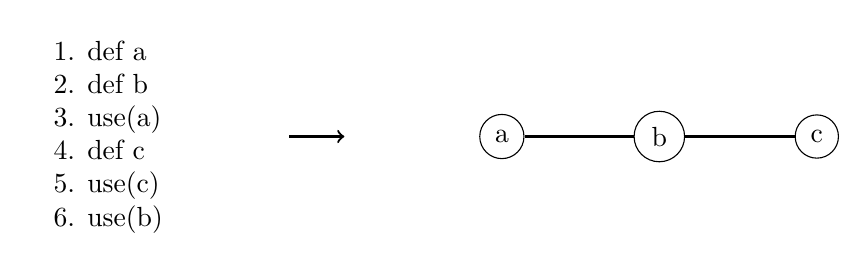
\begin{tikzpicture}
            \node at (0, 0) {\begin{tabular}{l}
                1. def a \\
                2. def b \\
                3. use(a)\\
                4. def c \\
                5. use(c)\\
                6. use(b)
            \end{tabular}};

            \draw[->, thick] (2.3, 0) -- (3, 0);
        
            \node[circle, draw] (a) at (5, 0) {a};
            \node[circle, draw] (b) at (7, 0) {b};
            \node[circle, draw] (c) at (9, 0) {c};
        
            \draw[thick] (a) -- (b);
            \draw[thick] (b) -- (c);
        \end{tikzpicture}
    \caption{Пример построения графа зацепленности}
    \begin{tabular}{r @{: } l}
        \textbf{def} & Объявление переменной \\
        \textbf{use} & Использование переменной \\
    \end{tabular}
    \label{fig:ex1}
    \end{figure}

    % \begin{figure}
    % \centering
    % \begin{tikzpicture}
    %     \node[circle, fill=cyan!60!white, draw] (a) at (5, 0) {a};
    %     \node[circle, fill=magenta!60!white, draw] (b) at (7, 0) {b};
    %     \node[circle, fill=cyan!60!white, draw] (c) at (9, 0) {c};
        
    %     \draw[thick] (a) -- (b);
    %     \draw[thick] (b) -- (c);

    % \end{tikzpicture}
    % \caption{Раскрашенный граф}
    % \label{fig:ex1-color}
    % \end{figure}

В графе на рисунке~\ref{fig:ex1} присутствует ребро $(a, b)$, поскольку в точке 2 переменная $a$ \textit{жива}, однако ребра $(a, c)$ в графе нет,
поскольку в точке 4 для переменной $a$ отсутствует путь, проходящий через точку её использования.
    
\end{example}

Теперь докажем, что по произвольному графу можно построить программу, распределение регистров которой даст раскраску этого графа.

Пусть $V$ — множество переменных, $R$ — множество регистров.
Тогда существует отображение $\varphi : V \to R$, при котором выполняется следующее свойство:

$$\forall a, b \in V \text{, если } a \text{ и } b \text{ зацеплены, то } \varphi(a) \neq \varphi(b).$$

Если построить биективное отображение $\psi: R \to C$, где $C$ — множество цветов,
то раскраска графа $IG(V)$ определяется как $\zeta = \psi \circ \varphi$.

% Мысль закончилась

В статье~\cite{chaitin1982} Чайтин предложил следующий алгоритм построения кода на основе графа:

\begin{enumerate}
    \item Если в графе существует вершина $\text{NODE}_i$, то в исходном коде объявляется переменная с соответствующим
    названием.
    \item Если в графе присутствует ребро $(\text{NODE}_i, \text{NODE}_j)$, то в исходный код добавляется операция,
    использующая эти переменные, например суммирование, чтобы они не могли занимать один регистр.
\end{enumerate}

Этот метод не всегда эффективен. В некоторых случаях требуются дополнительные конструкции, такие как \textit{операторы ветвления},
чтобы задача раскраски графа сводилась к задаче распределения регистров. Рассмотрим пример, когда такие преобразования необходимы.

\begin{example}

    \begin{figure}[h]
        \centering
        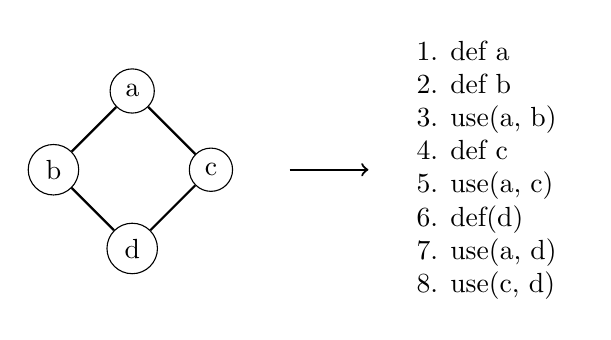
\begin{tikzpicture}
            \node at (6.5, 0) {\begin{tabular}{l}
                1. def a \\
                2. def b \\
                3. use(a, b) \\
                4. def c \\
                5. use(a, c) \\
                6. def(d) \\
                7. use(a, d) \\
                8. use(c, d)
            \end{tabular}};

            \draw[->, thick] (4, 0) -- (5, 0);
        
            \node[circle, draw] (a) at (2, 1) {a};
            \node[circle, draw] (b) at (1, 0) {b};
            \node[circle, draw] (c) at (3, 0) {c};
            \node[circle, draw] (d) at (2, -1) {d};
        
            \draw[thick] (a) -- (b);
            \draw[thick] (a) -- (c);
            \draw[thick] (b) -- (d);
            \draw[thick] (c) -- (d);
        \end{tikzpicture}
    \caption{Пример преобразования графа в код}
    \label{fig:ex2}
    \end{figure}

    На рисунке~\ref{fig:ex2} показано, что код, построенный по алгоритму, предложенному Чайтином, не всегда соответствует исходному графу.
    В данном случае в исходном коде наблюдается зацепленность переменных $a$ и $d$, хотя в исходном графе ребро $(a, d)$ отсутствует.
    Код, построенный на основе графа из рисунка~\ref{fig:ex2}, должен соответствовать изображению на рисунке~\ref{fig:right_ex2}.

    \begin{figure}
        \centering
        \lstset{basicstyle=\ttfamily\small, frame=single}
        \begin{lstlisting}
            01. def a
            02. if statement:
            03.     def b
            04.     use(a)
            05.     def d 
            06. else:
            07.     def c
            08.     use(a)
            09.     def d
            10. use(d)
        \end{lstlisting}
        \caption{Правильный вид исходного кода}
        \label{fig:right_ex2}
    \end{figure}
\end{example}

Алгоритм Чайтина легко исправляется следующим подходом:

\begin{enumerate} %% ??
    \item Для каждой вершины исходного графа создать переменную.
    \item Если между вершинами существует ребро, то создать \texttt{if statement}, в теле
    которого объявить эти переменные и использовать таким образом, чтобы они стали зацеплены.
\end{enumerate}
